\documentclass[main]{subfiles}

\begin{document}

\begin{example}
Suppose $1\mapsto k$ is an element in $Hom(\mathbb Z/n\mathbb Z,\mathbb Z/m\mathbb Z)$, then $m\mid kn\Rightarrow \dfrac{m}{(n,m)}$ divides $k\dfrac{n}{(n,m)}$, thus $\dfrac{m}{(n,m)}$ divides $k$, thus $k=\dfrac{im}{(n,m)}, i=0,\cdots,(n,m)-1$, thus $Hom(\mathbb Z/n\mathbb Z,\mathbb Z/m\mathbb Z)\cong\mathbb Z/(n,m)\mathbb Z$ \par
Consider $\mathbb Z/n\mathbb Z\otimes\mathbb Z/m\mathbb Z$, then $n(1\otimes1)=n\otimes1=0$, $m(1\otimes1)=1\otimes m=0$, thus $(n,m)(1\otimes1)=(rn+sm)(1\otimes1)=0$ \par
Apply functor $Hom(-,\mathbb Z/m\mathbb Z)$ to short exact sequence $0\to\mathbb Z\xrightarrow{\times m}\mathbb Z\to\mathbb Z/n\mathbb Z\to 0$, we get a left exact sequence $Hom(\mathbb Z/n\mathbb Z,\mathbb Z/m\mathbb Z)\to \mathbb Z/m\mathbb Z\xrightarrow{\times n} \mathbb Z/m\mathbb Z\to0$ \par
Apply functor $-\otimes\mathbb Z/m\mathbb Z$ to short exact sequence $0\to\mathbb Z\xrightarrow{\times m}\mathbb Z\to\mathbb Z/n\mathbb Z\to 0$, we get a left exact sequence $\mathbb Z/m\mathbb Z\xrightarrow{\times n} \mathbb Z/m\mathbb Z\to\mathbb Z/n\mathbb Z\otimes\mathbb Z/m\mathbb Z\to 0$ \par
And the kernel and cokernel of $\mathbb Z/m\mathbb Z\xrightarrow{\times n} \mathbb Z/m\mathbb Z$ are both $\mathbb Z/(n,m)\mathbb Z$
\end{example}

\begin{example}
$\mathbb Q/\mathbb Z\cong\bigoplus_{p}\mathbb Z\left[\dfrac{1}{p}\right]$
\end{example}

\begin{example}
$O(1,1)=\left\{\begin{pmatrix}
\cosh t&\sinh t \\
\sinh t&\cosh t
\end{pmatrix}\right\}$
\end{example}

\begin{example}\label{R^2=R}
$F$ is a field, $R=\End(F^\infty)=\{\text{infinite dimensional matrices}\}$, Consider $R\hookrightarrow R$ by embedding into odd rows and even rows, we have $R^2\cong R$ as right $R$ modules
\end{example}

\begin{example}
$GL(2,\mathbb F_2)=SL(2,\mathbb F_2)\cong S_3$
\end{example}

\begin{example}[A ring homomorphism between two local rings that isn't a local ring homomorphism]
$A=\left\{\dfrac{a}{b}\middle|a,b\in\mathbb Z,b\text{ odd}\right\}$ with maximal ideal $2A$, $B=\mathbb Q$, inclusion is not a local ring homomorphism
\end{example}

\begin{example}
$V\subseteq\mathbb A^n$ is an affine variety, $m\in\mathrm{Spm}k[V]$, $k[V]_{m}$ is the stalk of the sheaf of regular functions. Tow representatives $\frac{f}{u},\frac{g}{v}$ are of the same germ $\Leftrightarrow$ $\frac{f}{u}=\frac{g}{v}$ on $D(wuv)$ for some $w(m)\neq 0$ $\Leftrightarrow$ $w(fv-gu)=0$
\end{example}

\begin{example}[Multiplicative group scheme]
The multiplicative group scheme over $R$ is $\mathbb G_m=\Spec\mathbb R[x,x^{-1}]$, $\mathbb G_m(A)=\Hom(\mathbb R[x,x^{-1}],A)\cong A^\times, \phi_a\leftrightarrow a$, $\phi_a(x)=a$. The corresponding group multiplication $\mathbb G_m\times\mathbb G_m\xrightarrow m\mathbb G_m$ should be given by $\mathbb G_m(R)\times\mathbb G_m(R)\to\mathbb G_m(R)$, $(\phi_a,\phi_b)\mapsto\phi_{ab}$, which factors through $(\mathbb G_m\times\mathbb G_m)(R)\to\mathbb G_m(R)$, hence the corresponding comultiplication should be given by $\mathbb Z[x,x^{-1}]\xrightarrow\Delta\mathbb Z[x,x^{-1}]\otimes\mathbb Z[x,x^{-1}]$, $\Delta x=x\otimes x$, so that $\phi_a\otimes\phi_b(\Delta(x))=\phi_{ab}(x)$. By Yoneda's Lemma, this is the unique choice
\end{example}

\begin{example}[A surjective local homeomorphism may not be a covering]
$p:\mathbb R\setminus\{0\}\to S^1$, or $n$ sheeted cover with a point missing, $p$ is discrete but not proper
\end{example}

\begin{example}[Bundle with fiber isomorphic to vector space but not a vector bundle]
$E:=\displaystyle\bigsqcup_{x\in X}\mathbb R^n$
\end{example}

\begin{example}
$H'_n=H_{k+n}$ also defines a homology theory where the dimension axiom fails
\end{example}

\begin{example}[Hawaiian earring]\label{Hawaiian earring}
The \textbf{Hawaiian earring}\index{Hawaiian earring} $H$ is the union of circles with radius $\frac{1}{n}$ and centered at $(\frac{1}{n},0)$ with subspace topology in $\mathbb R^2$
\begin{center}
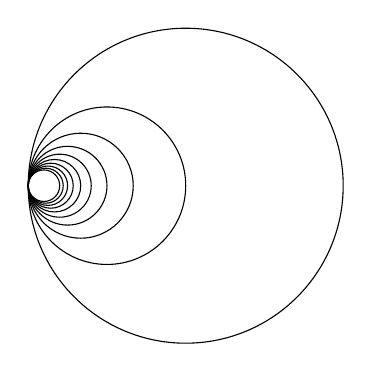
\begin{tikzpicture}[scale=2]
\foreach \x in {1,2,...,10}{
\draw ({1/\x},0) circle ({1/\x});
}
\end{tikzpicture}
\end{center}
\end{example}

\begin{proposition}
Hawaiian earring is not a CW complex since it is not locally contractible
\end{proposition}

\begin{example}[Topologist's sine curve]
The \textbf{topologist's sine curve}\index{topologist's sine curve} is
\[T=\left\{\left(x,\sin\left(\frac{1}{x}\right)\right)\middle|x\in(0,1]\right\}\cup\{(0,0)\}\]
\begin{center}
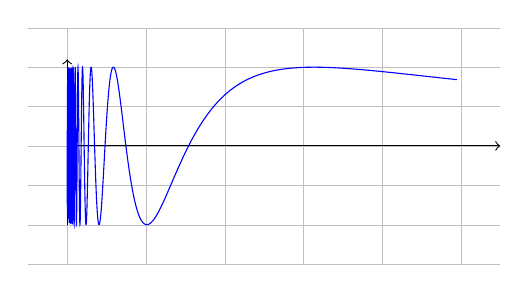
\begin{tikzpicture}[x=5cm]
\draw[xstep=.2,ystep=.5,lightgray,ultra thin] (-0.1,-1.5) grid (1.1,1.5);
\draw[->] (0,0) -- (1.1,0);
\draw[->] (0,-1) -- (0,1.1);
\draw[blue,domain=0.01:1,samples=5000] plot (\x-0.01, {sin((1/\x)r)});
\end{tikzpicture}
\end{center}
\end{example}

\begin{proposition}
The topologist's sine curve $T$ is connected but not path connected
\end{proposition}

\begin{example}[Warsaw circle]
The \textbf{Warsaw circle}\index{Warsaw circle} $W$ is the topologist's sine curve enclosed \par
Bijective map $W\to[0,1)$ is not a homeomorphism, thus not a quotient map. $W$ is weakly homotopic to a point but not homotopic
\end{example}

\begin{example}
$X=\mathbb N$ with discrete topology, $Y=\{0,1,\frac{1}{2},\frac{1}{3},\cdots\}$ with subspace topology of $\mathbb R$, then $f:X\to Y, n\mapsto\frac{1}{n}$ is a weak homotopy equivalence, however, $X,Y$ are not homotopy equivalent, otherwise suppose $g:X\to Y,h:Y\to X$ such that $hg\simeq1_X$, $gh\simeq1_Y$, suppose $F:Y\times I\to Y$ is a homotopy, then the restriction of $F$ on $\{y\}\times I$ must be a constant map since the connected components of $Y$ are just points, thus $F(y,0)=F(y,1)$, i.e. homotopic maps are in fact the same, for a similar argument on $X$, we have $hg=1_X$, $gh=1_Y$ , thus $h$ is injective which is impossible since $h^{-1}(h(0))$ consists of more then one point
\end{example}

\begin{example}\label{Cofibration counterexample}
$D^2=S^2\setminus\{N\}\subseteq S^2$ is not a cofibration. $D^2\setminus\{0\}\subseteq D^2$ is not a cofibration
\end{example}

\begin{example}\label{Mapping cylinder of inclusion may have different topology then induced subspace topology}
$A=[-1,0)\cup(0,1]$, $X=[-1,1]$, then the mapping cylinder of the inclusion $A\xhookrightarrow{i}X$ has different topology from the subspace topology $X\times\{0\}\cup A\times I$ induced from $X\times I$
\begin{center}
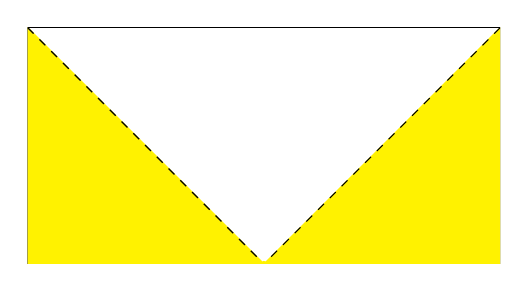
\begin{tikzpicture}[scale=3]
\clip (-1,0) rectangle (1,1);
\filldraw[yellow, ] (-1,0)--(-1,1)--(0,0);
\filldraw[yellow] (1,0)--(1,1)--(0,0);
\draw (-1,0)--(-1,1)--(1,1)--(1,0);
\draw[dashed](-1,1)--(0,0);
\draw[dashed](1,1)--(0,0);
\filldraw [yellow] (0,0) circle (0.01);
\end{tikzpicture}
\end{center}
\end{example}

\begin{example}\label{Nonclosed cofibration}
$\{a,b\}$ with trivial topology, $\{a\}\subseteq\{a,b\}$ is a nonclosed cofibration since there is a retraction $I\sqcup I\to I\sqcup\{0\}$, $(s,t)\mapsto(s,0)$
\end{example}

\begin{example}
The \textbf{comb space}\index{Comb space} is $[(0,0),(1,0)]\bigcup\bigcup_{n=1}^\infty[(\frac{1}{n},0),(\frac{1}{n},1)]$
\begin{center}
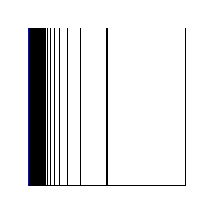
\begin{tikzpicture}[scale=2]
\draw(0,0)--(1,0);
\draw[blue](0,0)--(0,1);
\foreach \x in {1,2,...,100}{
\draw ({1/\x},0) -- ({1/\x},1);
}
\end{tikzpicture}
\end{center}
\end{example}

\begin{example}\label{A line with two origins}
A topological space with a cell decomposition may not be Hausdorff, consider $(-1,1)$ with two origins, which has $(-1,0),(0,1)$ as $1$ cells and two origins as $0$ cells
\begin{center}
\begin{tikzpicture}
\draw (-1,0)--(1,0);
\filldraw [fill=white, draw=black] (0,0) circle (0.03);
\filldraw [black] (0,0.5) circle (0.03);
\filldraw [black] (0,-0.5) circle (0.03);
\end{tikzpicture}
\end{center}
\end{example}

\begin{example}
$D\subseteq\mathbb C$ is the unit disc, $\displaystyle f(z)=\sum_{n=0}^\infty \frac{z^{2^n}}{n^2}$ is continuous on $\overline D$ and holomorphic on $D$ but not on any point on $\partial D$
\end{example}

\begin{example}[Tractrix]
An interval $I$ with one end point pushed or dragged along the $x$ axis gives a \textbf{Tractrix}\index{Tractrix}. The velocity has the same direction as $I$, i.e. $\displaystyle\frac{dx}{dy}=\pm\frac{\sqrt{a^2-y^2}}{y}$, which gives solution $\displaystyle x=\pm\left(\ln\frac{a+\sqrt{a^2-y^2}}{y}-\sqrt{a^2-y^2}\right)$
\begin{center}
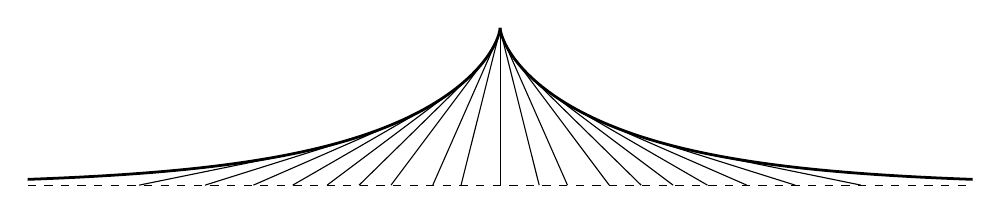
\begin{tikzpicture}[scale=2]
\clip (-3,0) rectangle (3,1);
\draw[line width=1, rotate=90, smooth,samples=100,domain=0.02:1] plot(\x,{ln((1+sqrt(1-(\x)^(2)))/(\x))-sqrt(1-(\x)^(2))});
\draw[line width=1, rotate=90, smooth,samples=100,domain=0.02:1] plot(\x,{-ln((1+sqrt(1-(\x)^(2)))/(\x))+sqrt(1-(\x)^(2))});
\draw[dashed](-3,0)--(3,0);
\draw[rotate=90] (0,0)--(1,0);
\foreach \x in {0.2,0.3,...,0.9,0.915,0.97}{
\draw[rotate=90] (\x,{ln((1+sqrt(1-(\x)^(2)))/(\x))-sqrt(1-(\x)^(2))})--(0,{ln((1+sqrt(1-(\x)^(2)))/(\x))-sqrt(1-(\x)^(2))+sqrt(1-(\x)^(2)))});
\draw[rotate=90] (\x,{-ln((1+sqrt(1-(\x)^(2)))/(\x))+sqrt(1-(\x)^(2))})--(0,{-ln((1+sqrt(1-(\x)^(2)))/(\x))+sqrt(1-(\x)^(2))-sqrt(1-(\x)^(2)))});
}
\end{tikzpicture}
\end{center}
\end{example}

\begin{example}
$R$ is a commutative ring. The category of $R$-modules is a monoidal category with
\begin{itemize}
\item $(A\otimes B)\otimes C\xrightarrow{\alpha} A\otimes (B\otimes C)$, $(a\otimes b)\otimes c\mapsto a\otimes (b\otimes c)$
\item $R\otimes A\xrightarrow{\lambda}A$, $r\otimes a\mapsto ra, A\otimes R\xrightarrow{\rho}A$, $a\otimes r\mapsto ra$
\end{itemize}
\end{example}

\begin{example}
$R$ is a commutative ring. $R$-algebra/coalgebra/bialgebra is a monoid/comonoid/bimonoid of the category of $R$-modules, 
\end{example}

\begin{example}
The image of a functor is not necessarily a category \par
Consider the following categories $\mathscr C$ and $\mathscr D$
\begin{center}
\begin{tikzcd}
A \arrow[r, "f"] \arrow["1_A"', loop, distance=2em, in=125, out=55] & B \arrow["1_B"', loop, distance=2em, in=125, out=55] & C \arrow[r, "g"] \arrow["1_C"', loop, distance=2em, in=125, out=55] & D \arrow["1_D"', loop, distance=2em, in=125, out=55]
\end{tikzcd}
\end{center}
\begin{center}
\begin{tikzcd}
E \arrow[r, "h"] \arrow["1_E"', loop, distance=2em, in=125, out=55] \arrow[rr, "ih", bend right] & F \arrow["1_F"', loop, distance=2em, in=125, out=55] \arrow[r, "i"] & G \arrow["1_G"', loop, distance=2em, in=125, out=55]
\end{tikzcd}
\end{center}
Consider functor $F:\mathscr C\to\mathscr D$, $F(A)=E$, $F(B)=F$, $F(C)=F$, $F(D)=G$, $F(f)=h$, $F(g)=i$
\end{example}

\begin{example}[Presheaves that are not sheaves]
\begin{enumerate}
\item $G$ is a nontrivial abelian group. Consider presheaf $\mathcal G$ given by $\mathcal G(U)=G$ for any nonempty open subset and $\mathcal G(\varnothing)=0$. For example $G=\mathbb Z/2$, $X=\{a,b\}$ with discrete topology, $\mathcal G(\{a,b\})=\mathcal G(\{a\})=\mathcal G(\{b\})=\mathbb Z/2$, $\mathcal G(\varnothing)=0$. Then $1$ on $\{a\}$ and $0$ on $\{b\}$ cannot be glued together.
\item Suppose $\phi:\mathcal F\to\mathcal G$ is a morphism of sheaves, $\im\phi$ and $\coker\phi$ are not generally sheaves. For example consider $\exp:\mathcal O\to\mathcal O^\times$, $\im\exp$ is a presheaf but not a sheaf
\end{enumerate}
\end{example}

\begin{definition}[$\mathcal O(n)$ bundle over Riemann sphere $S^2\cong\mathbb CP^1$]
Suppose $\left(\mathbb C, z\mapsto z\right)$, $\left(S^2\setminus 0, z\mapsto\dfrac{1}{z}\right)$ are the charts coordinate of $S^2$ with transition map $z\mapsto \dfrac{1}{z}$ both ways on $\mathbb C\setminus 0$, or equivalently \par
$\left(U_0,[1,z]\mapsto z\right)$, $\left(U_1,[z,1]\mapsto z\right)$ are the corresponding charts of $\mathbb CP^1$ with transition map $z\mapsto\dfrac{1}{z}$ both ways on $U_0\cap U_1$, namely, $S^2\to\mathbb CP^1$, $z\mapsto [1,z]$, $\infty\mapsto[0,1]$ is and isomorphism because of isomorphisms on charts \par
Now define $\mathcal{O}(n)$ line bundle on $S^2$ by specify transition functions $g_{10}(z)=z^{-n}$, $g_{01}(z)=z^n$, $\forall z\in \mathbb C\setminus0\cong U_0\cap U_1$ \par
\end{definition}

\begin{definition}[Tautological line bundle over Riemann sphere]
The tautological bundle\index{Tautological bundle} is $\mathcal{O}(-1)$, tautological bundle is defined as a subspace $E$ of $\mathbb CP^1\times\mathbb C^2$ consists of $(l,v)$ with $v\in l$ projects to the first factor, let's figure out the trivializations! \par
$\varphi_0: U_0\times\mathbb C^2\cap E\to\mathbb C\times\mathbb C$, $([1,z],t(1,z))\mapsto(z,t)$, and $\varphi_1: U_1\times\mathbb C^2\cap E\to\mathbb C\times\mathbb C$, $([z,1],t(z,1))\mapsto(z,t)$, since $\varphi_1\circ\varphi_0^{-1}: (U_0\cap U_1)\times\mathbb C^2\cap E\to(U_0\cap U_1)\times\mathbb C^2\cap E$, $(z,t)\mapsto\left(\dfrac{1}{z},zt\right)$, the transition function $g_{10}(z)=z$ \par
\end{definition}

\begin{remark}
$\mathcal{O}(-1)$ doesn't nonzero global section, suppose $s$ is a global section of $\mathcal{O}(-1)$, then $s(x)=(x,f(x))\in E\hookrightarrow\mathbb CP^1\times\mathbb C^2$ is holomorphic, but then image of $\sigma$ has to be a point, and this point must be zero\par
\end{remark}

\begin{example}
We still use $U_0,U_1$ to denote coordinate charts, $\varphi_0,\varphi_1$ to denote corresponding trivializations \par
Global sections of $\mathcal{O}=\mathcal{O}(0)$ are exactly holomorphic functions which are just constants, suppose $s: S^2\to \mathcal{O}$ is a section, and $\varphi_0\circ s|_{U_0}(z)=(z,f_0(z))$, $\varphi_1\circ s|_{U_1}\left(\dfrac{1}{z}\right)=\left(\dfrac{1}{z},f_1\left(\dfrac{1}{z}\right)\right)$, then we have $(z,f_1(z))=\varphi_1\circ s|_{U_1}(z)=\varphi_1\circ s|_{U_0}(z)=\varphi_1\circ\varphi_0^{-1}\circ\varphi_0\circ s|_{U_0}(z)=\varphi_1\circ\varphi_0^{-1}(z,f_0(z))=(z,g_{10}(z)f_0(z)), \forall z\in U_0\cap U_1$,
thus $f_1(z)=g_{10}(z)f_0(z)=f_0(z)$ which precisely means $s$ correspond to holomorphic function $f$ over $X$, $f|_{U_0}=f_0, f|_{U_1}=f_1$ \par
Let's show that the canonical bundle(which in the case of a Riemann surface is the same as the cotangent bundle) is $\mathcal{O}(-2)$, since $d\left(\dfrac{1}{z}\right)=-\dfrac{1}{z^2}dz$, the transition function would be $g_{10}(z)=-z^{2}$, but using $dz$ or $-dz$ as the a basis element would be isomorphic
\end{example}

\begin{proposition}
$H^0\left(CP^1,\mathcal{O}(n)\right)$, the vector space of global sections of $\mathcal{O}(n)\to\mathbb CP^1,n\geq0$  generated by homogeneous polynomials $z_0^n,z_0^{n-1}z_1,\cdots,z_0z_1^{n-1},z_1^{n}$
\end{proposition}

\begin{proof}
$z_0^kz_1^{n-k}$ have the forms $z_1^{n-k}$ and $z_0^k$ in $U_0$ and $U_1$
\end{proof}

\begin{example}[Line bundles on the projective space $\mathbb CP^n$]
Suppose $\left(U_0,[1,z_1,\cdots,z_n]\mapsto(z_1,\cdots,z_n)\right)$, $\left(U_n,[z_0,z_1,\cdots,z_{n-1},1]\mapsto(z_0,\cdots,z_{n-1})\right)$ be coordinate charts of $\mathbb CP^n$, with transition map $U_i\cap U_j\to U_i\cap U_j, \left(\dfrac{z_0}{z_i},\cdots,\widehat{\dfrac{z_i}{z_i}},\cdots,\dfrac{z_n}{z_i}\right)\mapsto\left(\dfrac{z_0}{z_j},\cdots,\widehat{\dfrac{z_j}{z_j}},\cdots,\dfrac{z_n}{z_j}\right)$, which is kind of like multiply by $\dfrac{z_i}{z_j}$, then the line bundle $\mathcal{O}(m)$ is defined by transition function $g_{ji}=\dfrac{z_j}{z_i}$ which satisfies the cocycle condition \par
Similarly, we can check that the tautological bundle $E=\left\{(l,v)\middle| v\in l\right\}\subset\mathbb CP^n\times\mathbb C^{n+1}$ projects to $\mathbb CP^n$ is $\mathcal{O}(1)$ \par
It is obvious that any degree $n$ polynomial are global section of $\mathcal{O}(n)$
\end{example}

\begin{example}
$X$ is topological space, $End(X)$ is a unital nonassociative $\mathbb R$ algebra which is not symmetric, antisymmetric, nor does it satisfy Jacobi identity
\end{example}

\begin{example}
Consider $C^\infty(M)$ where $M$ is a smooth manifold, then $\mathcal{L}(M)=Der(C^\infty(M))$ consists of vector fields, it is a Lie algebra, hence we can think of derivations as linear differential operator of order $1$, then we know that the commutator of two such operators is again a linear differential operator of order $1$
\end{example}

\begin{example}
Let $\mathfrak{g}$ be a Lie algebra, then ideals of $\mathfrak{g}$ precisely the Lie algebra subrepresentations of the adjoint representation $(ad,\mathfrak{g})$
\end{example}

\begin{example}[Lie algebra of $M_n(\mathbb R)$]
Suppose $X=\displaystyle\sum_{i,j}X_{ij}\dfrac{\partial}{\partial x_{ij}}$ is a left invariant
\begin{align*}
X_{kl}(A)&=\sum_{i,j}X_{ij}(A)\dfrac{\partial x_{kl}}{\partial x_{ij}}(A) \\
&=X_A(x_{kl})=(L_A)_0X_0(x_{kl}) \\
&=X_0(x_{kl}\circ L_A) \\
&=\sum_{i,j}X_{ij}(0)\dfrac{\partial (x_{kl}\circ L_A)}{\partial x_{ij}}(0) \\
&=X_{kl}(0)
\end{align*}
Thus $X_{ij}$ are constants
\begin{align*}
[X,Y]&=\displaystyle\left[\sum_{i,j}X_{ij}\dfrac{\partial}{\partial x_{ij}},\sum_{k,l}Y_{kl}\dfrac{\partial}{\partial x_{kl}}\right] \\
&=\sum_{i,j,k,l}X_{ij}Y_{kl}\left[\dfrac{\partial}{\partial x_{ij}},\dfrac{\partial}{\partial x_{kl}}\right] \\
&=\sum_{i,j}X_{ij}Y_{ij}\left[\dfrac{\partial}{\partial x_{ij}},\dfrac{\partial}{\partial x_{kl}}\right] \\
&=0
\end{align*}
Therefore $\mathrm{Lie}(M_n(\mathbb R))=0$
\end{example}

\begin{example}[Lie algebra of $GL(n,\mathbb R)$]
Suppose $X=\displaystyle\sum_{i,j}c_{ij}\dfrac{\partial}{\partial x_{ij}}$ is a left invariant field
\begin{align*}
c_{kl}(A)&=\sum_{i,j}c_{ij}(A)\dfrac{\partial x_{kl}}{\partial x_{ij}}(A) \\
&=X_A(x_{kl})=(L_A)_IX_I(x_{kl}) \\
&=X_I(x_{kl}\circ L_A) \\
&=\sum_{i,j}c_{ij}(I)\dfrac{\partial (x_{kl}\circ L_A)}{\partial x_{ij}}(I) \\
&=\sum_{i}a_{ki}c_{il}(I)
\end{align*}
Hence $C(A)=AC(I)$, $\dfrac{\partial c_{kl}}{\partial x_{ij}}=\delta_{ki}c_{jl}(I)$
\begin{align*}
[X,Y]&=\displaystyle\left[\sum_{i,j}c_{ij}\dfrac{\partial}{\partial x_{ij}},\sum_{k,l}d_{kl}\dfrac{\partial}{\partial x_{kl}}\right] \\
&=\sum_{i,j,k,l}\left[c_{ij}\dfrac{\partial}{\partial x_{ij}},d_{kl}\dfrac{\partial}{\partial x_{kl}}\right] \\
&=\sum_{i,j,k,l}c_{ij}\dfrac{\partial}{\partial x_{ij}}\left(d_{kl}\dfrac{\partial}{\partial x_{kl}}\right)-d_{kl}\dfrac{\partial}{\partial x_{kl}}\left(c_{ij}\dfrac{\partial}{\partial x_{ij}}\right) \\
&=\sum_{i,j,k,l}c_{ij}\left(\dfrac{\partial d_{kl}}{\partial x_{ij}}\dfrac{\partial}{\partial x_{kl}}+d_{kl}\dfrac{\partial^2}{\partial x_{ij}\partial x_{kl}}\right)-d_{kl}\left(\dfrac{\partial c_{ij}}{\partial x_{kl}}\dfrac{\partial}{\partial x_{ij}}+c_{ij}\dfrac{\partial^2}{\partial x_{ij}\partial x_{kl}}\right) \\
&=\sum_{i,j,k,l}c_{ij}\dfrac{\partial d_{kl}}{\partial x_{ij}}\dfrac{\partial}{\partial x_{kl}}-d_{kl}\dfrac{\partial c_{ij}}{\partial x_{kl}}\dfrac{\partial}{\partial x_{ij}} \\
&=\sum_{i,j,k,l}c_{ij}\dfrac{\partial d_{kl}}{\partial x_{ij}}\dfrac{\partial}{\partial x_{kl}}-\sum_{i,j,k,l}d_{kl}\dfrac{\partial c_{ij}}{\partial x_{kl}}\dfrac{\partial}{\partial x_{ij}} \\
&=\sum_{i,j,k,l}c_{ij}\dfrac{\partial d_{kl}}{\partial x_{ij}}\dfrac{\partial}{\partial x_{kl}}-\sum_{i,j,k,l}d_{ij}\dfrac{\partial c_{kl}}{\partial x_{ij}}\dfrac{\partial}{\partial x_{kl}} \\
&=\sum_{i,j,k,l}\left(c_{ij}\dfrac{\partial d_{kl}}{\partial x_{ij}}-d_{ij}\dfrac{\partial c_{kl}}{\partial x_{ij}}\right)\dfrac{\partial}{\partial x_{kl}} \\
&=\sum_{j,k,l}\left(c_{kj}d_{jl}-d_{kj}c_{jl}\right)\dfrac{\partial}{\partial x_{kl}} \\
&=\sum_{k,l}\left(\sum_{j}c_{kj}d_{jl}-d_{kj}c_{jl}\right)\dfrac{\partial}{\partial x_{kl}} \\
&=\sum_{k,l}b_{kl}\dfrac{\partial}{\partial x_{kl}}
\end{align*}
Here $B=[C,D]$. Therefore $\mathrm{Lie}(GL(n,\mathbb R))=\mathfrak{gl}(n,\mathbb R)$
\end{example}

\begin{example}
Consider the $\Phi:GL(n,\mathbb R)\to M_n(\mathbb R),A\mapsto A^TA$ which is a smooth map, and level set $\Phi^{-1}(I)=O(n,\mathbb R)$ is the orthogonal group, to show this is a Lie subgroup, thanks to Theorem \ref{Constant rank level set theorem}, it suffices to show $\Phi$ is of constant rank, but $\Phi$ is equivariant assuming $GL(n,\mathbb R)$ acts on itself by right multiplication and acts on $M_n(\mathbb R)$ by $X\cdot A=A^TXA,X\in M_n(\mathbb R),A\in GL(n,\mathbb R)$, since $\Phi(A)\cdot B=B^TA^TAB=\Phi(AB)$ \par
$(d\Phi)_I(B)=B^T+B$, and $T_I(O(n,\mathbb R))=\ker(d\Phi)_I=\{B\in M(n,\mathbb R)|B^T+B=0\}$
\end{example}

\begin{example}
Union of topologies may not be a topology
\end{example}

\end{document}